% AnchorMTM 全文中文翻译（与 main.tex 第 3 版逐句对应，2026-11-03）
% 编译：tectonic -X compile main_zh.tex   （XeLaTeX，系统字体 STSong / Hiragino Sans GB / STHeiti）
\documentclass[fontset=none,zihao=5,a4paper]{ctexart}
\setCJKmainfont{STSong}[BoldFont=STHeiti]
\setCJKsansfont{Hiragino Sans GB}
\setCJKmonofont{STHeiti}
\usepackage[margin=2.2cm]{geometry}
\usepackage{amsmath,amssymb,amsthm}
\usepackage{graphicx,booktabs,url}
\usepackage[ruled,vlined]{algorithm2e}
\usepackage[hidelinks]{hyperref}
\usepackage{caption}
\captionsetup{font=small,labelfont=bf}
\SetAlFnt{\small}
\DontPrintSemicolon
\renewcommand{\algorithmcfname}{算法}
\SetKwInput{KwData}{输入}
\SetKwInput{KwResult}{输出}
\SetKw{KwReturn}{返回}
\newtheorem{theorem}{定理}
\newtheorem{proposition}{命题}
\renewcommand{\proofname}{证明}
\newcommand{\dtop}{d_{\mathrm{top}}}
\newcommand{\lca}{\operatorname{lca}}
\newcommand{\nroe}{\mathrm{NROE}}
\newcommand{\pos}[1]{\left[#1\right]^+}
\newcommand{\abovecaptionskipzh}{}
\ctexset{section={format=\Large\bfseries\raggedright},subsection={format=\large\bfseries\raggedright},subsubsection={format=\normalsize\bfseries\raggedright}}
\title{AnchorMTM：时变标量场的空间锚定合并树图\\[4pt]\large （中文翻译稿，对应英文稿第 3 版，2026-11-03）}
\author{匿名作者}
\date{}
\begin{document}
\maketitle

\begin{figure}[h]
\centering
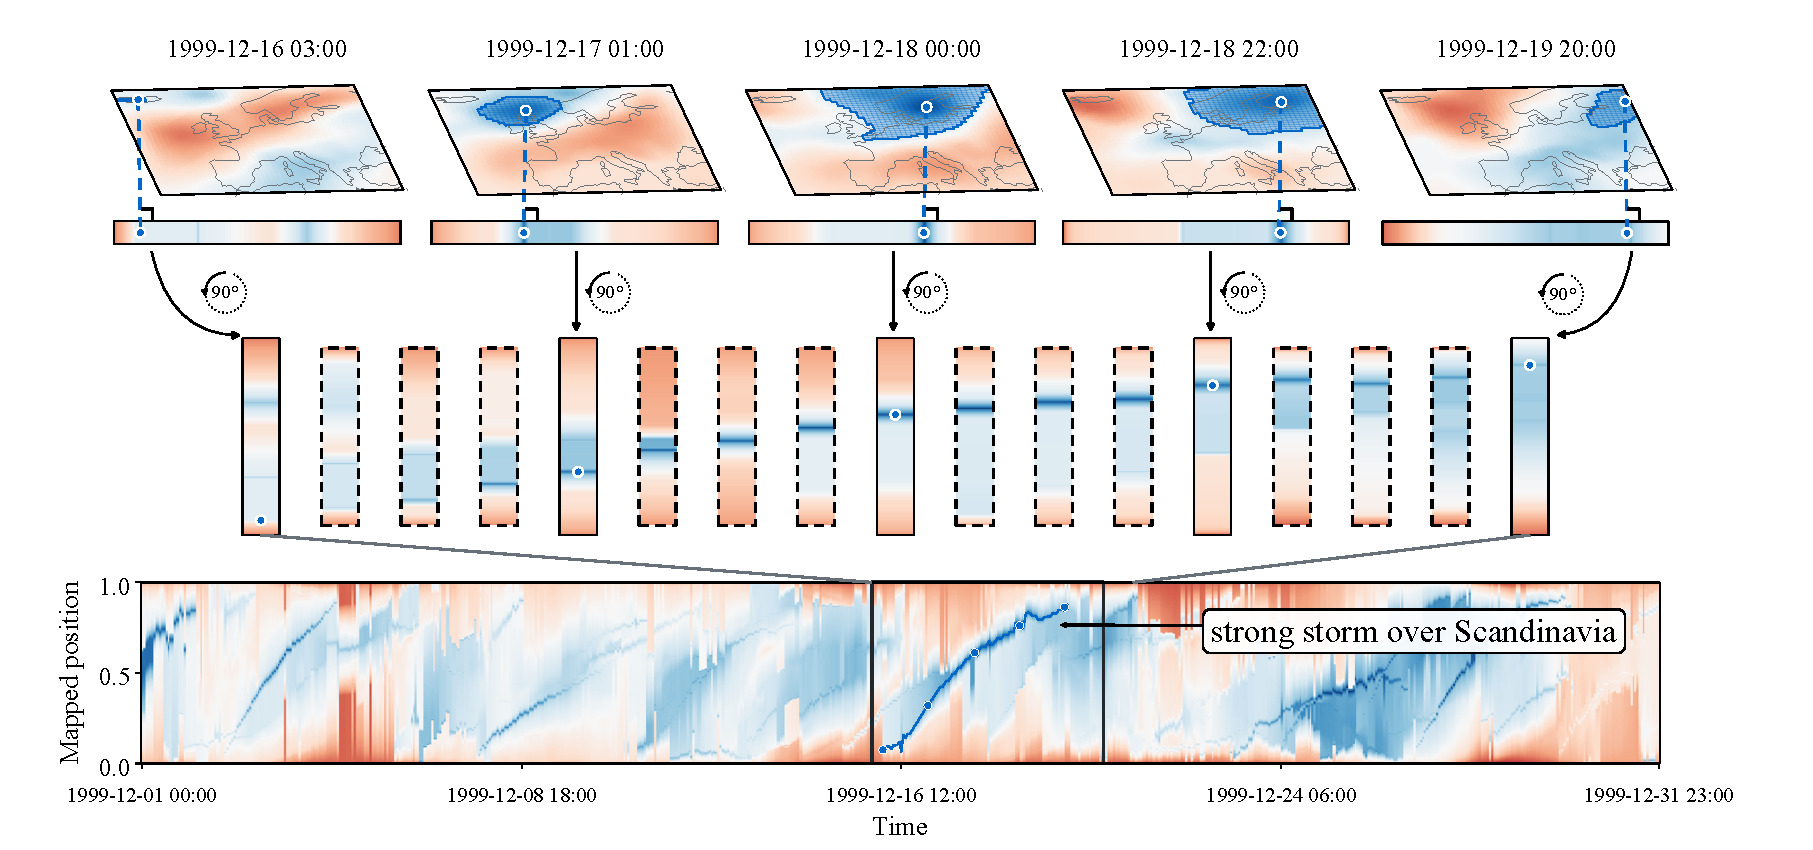
\includegraphics[width=\linewidth]{figures/anchor_storms_overview.pdf}
\caption{Storms 示例：把空间特征支撑与时间地图联系起来（$\varepsilon=5\%$）。上：一个匹配极值的五个快照及其标量剖面；蓝色轮廓标出其叶弧支撑，虚线引导线把极值连到它在剖面中的锚点。中：旋转 $90^\circ$ 后的剖面；虚线边框表示采样的中间帧。下：完整的 744 帧地图，框出与风暴相关的区域，蓝色标出该匹配特征的显示位置。}
\label{fig:storms_overview}
\end{figure}

\begin{abstract}
时间合并树图在一张图中概括不断演化的标量拓扑，但其显示轴不一定对应任何空间方向。我们把合并树图统一表述为一个约束布局问题：叶序的合并值误差不超过给定容许量，区间布局受位置上限约束，目标函数由多项组成；TMTM 和 ST-MTM 都是其中的精确拓扑特例。在这一框架内，AnchorMTM 把显示轴锚定到一个固定的空间参考上，这个参考由匹配极值的运动一次性估计得到，也可以给定；它只暴露一个控制量，即合并误差预算 $\varepsilon$：精确模式保持合并树不变，预算模式用一个声明的合并值误差换取位置。地图由带最优合并屏障的拓扑预算叶序搜索和一个带上限的二次规划构造。三个可证明的界给出精确拓扑、有限宽度和有限拓扑误差各自造成的不可避免的位移；它们只依赖约束，因此同样可以衡量已有的地图。在七个平面和体数据序列（917 帧）上，TMTM 和 ST-MTM 的顺序误差有 54--95\% 是可以避免的；精确模式在每个平面序列上与下界相差不超过 0.03 个百分点，且合并树不变；$\varepsilon$ 描出位置–拓扑权衡曲线，每张渲染出的地图都在其容许量之内。

\noindent\textbf{关键词：}时变标量场，合并树图，空间锚定，拓扑保持，约束布局。
\end{abstract}

\section{引言}
二维和三维时变标量场描述了气压系统、燃烧结构和流动特征等不断演化的现象。
分析它们需要理解特征出现在哪里、它们沿某个相关空间方向如何运动，以及它们的层次关系在整个序列中如何变化。
极值和连通分量的合并描述了这种不断演化的标量结构，而空间坐标把它与物理区域联系起来。
一个时间概览应当把这些方面结合在一起。
图~\ref{fig:storms_overview} 展示了空间支撑和参考位置如何与标量剖面以及最终的时间地图相联系。

动画保留了每一时刻的空间视图，但比较相距较远的时刻需要来回浏览和记忆。
小多图同时呈现所有观测，代价是占用屏幕空间。
静态时间概览把一个显示轴分配给时间，把空间区域压缩到另一个轴上~\cite{Tversky:2002:Animation,Robertson:2008:Animation,Bach:2017:STC}。
空间线性化让长序列可以在一张图中看到；其一维坐标的含义决定了这张概览能回答哪些空间问题。

合并树图围绕标量特征及其层次来组织这种压缩。
时间合并树图（TMTM）把增广合并树线性化为在时间上对齐的标量剖面~\cite{Koepp:2023:TMTM}。
极小值和其间的屏障编码了极值和合并值，揭示了标量结构及其时间演化。
时空合并树图（ST-MTM）把相对空间距离和时间位置约束纳入一个几何感知的布局~\cite{STMTM:2026}。
这些方法为时间标量拓扑的紧凑概览奠定了基础。

为层次、相对距离或时间对齐而选择的显示坐标，不一定对应一个固定的物理方向。
这时它的位置不能直接读作经度或沿流动轴的距离，它的变化也不一定代表沿该方向的运动。
相对几何提供了空间关系，但没有确定绝对坐标的原点。
剩下的问题是：如何在保留层次信息的同时，给时间地图一个一致的空间参考。

我们提出\emph{自动空间锚定}：用整个序列中匹配的极值估计一个主导运动方向，在这个共同坐标系中分配投影目标，并在约束允许的范围内把显示锚点放在目标附近。
也可以改用针对具体任务的物理方向。
方向估计是标准的主特征向量计算；我们的贡献在于把它与合并树布局、显式的拓扑预算和位置界联系起来。
当不同子树的投影叶子相互交错，而精确拓扑要求子树占据连续的叶块时，参考顺序就会与拓扑冲突。
有限的特征宽度引入进一步的装箱约束。
允许有限的拓扑误差可以解除一部分排序限制，从而揭示出一个可控的位置–拓扑权衡。

AnchorMTM，即\emph{空间锚定合并树图}，遵循一个构造流程：提取并匹配特征，构造固定参考，寻找满足拓扑要求的叶序，在合法区间内优化锚点，并在共同的时间轴上重建标量剖面。
精确模式和预算模式使用同一个布局框架，只是允许的合并误差不同。
位置界则解释了拓扑和有限宽度造成的不可避免的偏差。

我们的主要贡献如下：
\begin{itemize}
\item 我们把合并树图表述为带合并值容许量、位置上限和复合目标函数的层次约束区间布局；TMTM、ST-MTM、参考投影和 AnchorMTM 都是这一表述的特例。
\item 我们提出 AnchorMTM：通过固定参考、带最优合并屏障的拓扑预算叶序和带上限的锚点优化，赋予显示轴空间含义，并由单一的合并误差预算控制。
\item 我们建立三个可证明的位置界，它们对满足其假设的所有特例都成立；并在七个序列上表明，已有地图的顺序误差大部分是可以避免的。
\end{itemize}

\section{相关工作}\label{sec:related}
\subsection{有空间参考的时间可视化}
静态时间显示同时呈现相距较远的观测，而动画保留每一时刻的空间视图；二者的用处取决于分析任务~\cite{Tversky:2002:Animation,Robertson:2008:Animation}。
广义时空立方体描述了连接这些视图的变换~\cite{Bach:2017:STC}。
在压缩的时间概览中，空间坐标决定了哪些位置和运动关系仍能被直接解读。

Hovmöller 图保留一个选定的物理坐标，并对其他维度做概括~\cite{Hovmoller:1949}。
地理排序和空间填充曲线则遍历整个区域~\cite{Guo:2006:SpatialOrder,Dafner:2000:CSFC}。
Dynamic Volume Lines 和数据驱动的曲线把空间遍历扩展到体数据比较和标量感知的排序~\cite{Weissenboeck:2019:DVL,Zhou:2021:DSF}。
遍历可以保留空间邻域，但其一维坐标通常不同于一个固定投影，而且仅靠遍历邻接并不能保证合并层次。

一维投影可以组织时空现象~\cite{Franke:2021:1DP}，MotionRugs 揭示移动实体的群体行为~\cite{Buchmueller:2019:MR}。
更一般地，一个嵌入是在原始区域的关系与其显示组织之间做权衡~\cite{Nonato:2019:MP}。
相对邻近并不能确定绝对坐标。
AnchorMTM 为拓扑特征分配固定的投影目标，并在层次约束和区间约束下量化它们的位移，从而把空间参考与时间拓扑概览结合起来。

\subsection{基于拓扑的时间地图与几何感知布局}
基于拓扑的可视化通过连通性组织标量结构~\cite{Heine:2016:Survey}。
地形图和地形剖面通过地形或一维标量表示来表达层次~\cite{Weber:2007:TL,Oesterling:2013:TLP}，并有保持几何和保持时间连贯的扩展~\cite{Beketayev:2012:GPTL,Herick:2020:TCTL}。
这些表示在紧凑的视图中把标量值与特征关系联系起来。

TMTM 在静态合并树图中强调拓扑特征的完整和时间对齐~\cite{Koepp:2023:TMTM}。
ST-MTM 纳入了相对空间几何和时间位置约束~\cite{STMTM:2026}。
这些侧重点让空间关系和连贯性在地图中发挥作用，但其显示坐标仍可以不同于一个固定的物理方向。
AnchorMTM 从极值运动估计一个共同方向（或接受一个物理方向），并把这个参考与拓扑预算布局和可证明的位置界结合起来。
它沿用了已有的剖面和标量填充基础。

受层次约束的叶序选择传统上最小化相邻元素的差异~\cite{BarJoseph:2001:OLO}；按目标顺序重排的研究考虑了相关的树一致排列~\cite{Bulteau:2022:RT}。
带分离约束的布局控制几何重叠和位移~\cite{Dwyer:2006:IPSEP,Li:2019:SOI}。
AnchorMTM 把这些布局问题与固定的空间目标结合起来。
其精确拓扑下的点叶序界有闭式解，而有限宽度下的候选排序仍是启发式的。

合并树比较取决于所用的描述子和对应关系~\cite{Yan:2021:Survey}。
带标签的同表型/交错比较支持固定身份下的合并值核算~\cite{Munch:2019:LINF,Gasparovic:2024:IID}，有序合并树把标量曲线与单调交错距离联系起来~\cite{Beurskens:2025:OMT}。
我们用固定标签来测量显示出的合并误差。
最优屏障子问题与极小极大超度量拟合有关~\cite{Farach:1995:RM}，额外的限制是所有显示出的合并都由一个线性顺序诱导。

\section{背景}\label{sec:background}
\subsection{增广合并树与特征支撑}
对于采样的二维或三维场 $f_t:D\to\mathbb{R}$，合并树 $T_t$ 记录下水平集的连通性：随着阈值增大，极小值产生连通分量，鞍点把它们连接起来。
对场取负得到分裂树的约定。
临界点是超结点，由超弧连接；增广把正则顶点关联到这些弧上~\cite{Koepp:2023:TMTM,STMTM:2026,Tierny:2018:TTK}。
提取和简化在布局之前完成。

一片叶子代表位于空间位置 $p_i^t$ 的一个极值。
其特征支撑 $S_i^t$ 由该极值及其所在叶弧上的正则采样点组成，不包括父临界采样点。
它不是完整的连通分量，也不是该弧以上的整棵子树。
为了做跨帧重叠，这些支撑是稳定空间采样 ID 的集合：同一个 ID 在各帧中必须表示同一个空间采样点。
固定网格的输入通过一致的采样编号保持这种身份。
内部弧保留更多正则采样点，用于标量填充。
记 $\mathcal{D}_t(v)$ 为结点 $v$ 的后代叶子标签，$h_t(v)$ 为其标量值。
最近公共祖先决定合并高度矩阵：
\begin{equation}\label{eq:merge}
 V_{ij}^t=h_t(\lca(i,j)),\quad i\ne j;\qquad
 V_{ii}^t=f_t(p_i^t).
\end{equation}
同一高度的合并事件构成一个多叉结点；任意的二叉细化不会增加严格约束。
后面的所有保证都针对所提供的（可能已简化的）树。

\subsection{一维合并树剖面}
一维合并树剖面在选定的叶序中把极值放在锚点上。
叶弧上的正则顶点在叶区间内提供标量背景；内部弧和到最近公共祖先的路径填充其间的间隙~\cite{Koepp:2023:TMTM,STMTM:2026}。
在并树约定下，极值成为剖面的极小值，两个锚点之间剖面的最大值就是它们显示出的合并值。
精确保持要求每棵严格子树占据一个连续的叶块。
把这些剖面沿时间排列，就得到一张静态时间地图。
这个剖面模型是下面空间锚定公式的基础。

\section{AnchorMTM}\label{sec:method}
AnchorMTM 把一个共同的空间参考与显示的叶锚点联系起来。
我们先构造参考并给出布局公式，再描述构造过程，最后通过可证明的界解释其不可避免的位置代价。
分析采用并树约定；分裂树的标量符号在重建后恢复。

\subsection{空间参考与问题表述}
\paragraph{跨帧叶对应。}
我们用叶弧支撑 $S_i^t$ 来跟踪合并树的叶极值 $p_i^t$。
在一个共享的固定网格上，基于重叠的预处理~\cite{STMTM:2026}统计共同的空间采样点：
\begin{equation}\label{eq:overlap}
 O_{ij}^t=|S_i^t\cap S_j^{t+1}|.
\end{equation}
匈牙利算法在一对一配对上最大化总交集数，并丢弃零重叠的配对。
目标不是交并比（IoU）。
图~\ref{fig:leaf_correspondence} 展示了由此得到的身份状态。

\emph{延续}继承一个轨迹 ID；\emph{出生/消亡}开始一个未匹配的当前身份，或结束一个未匹配的先前轨迹。
对于\emph{非双射的对应}，包括可能的一对多、多对一和模糊关系，只保留被分配的一对一链接。
这些身份状态既不识别物理上的分裂/合并事件，也不构成分支谱系。
对当前叶 $i$，$\mu_t(i)$ 表示其有效的前驱。
布局接收与叶行对齐的预计算轨迹；上游的支撑和置信度约定在补充材料中详述。

\begin{figure}[tbp]
\centering
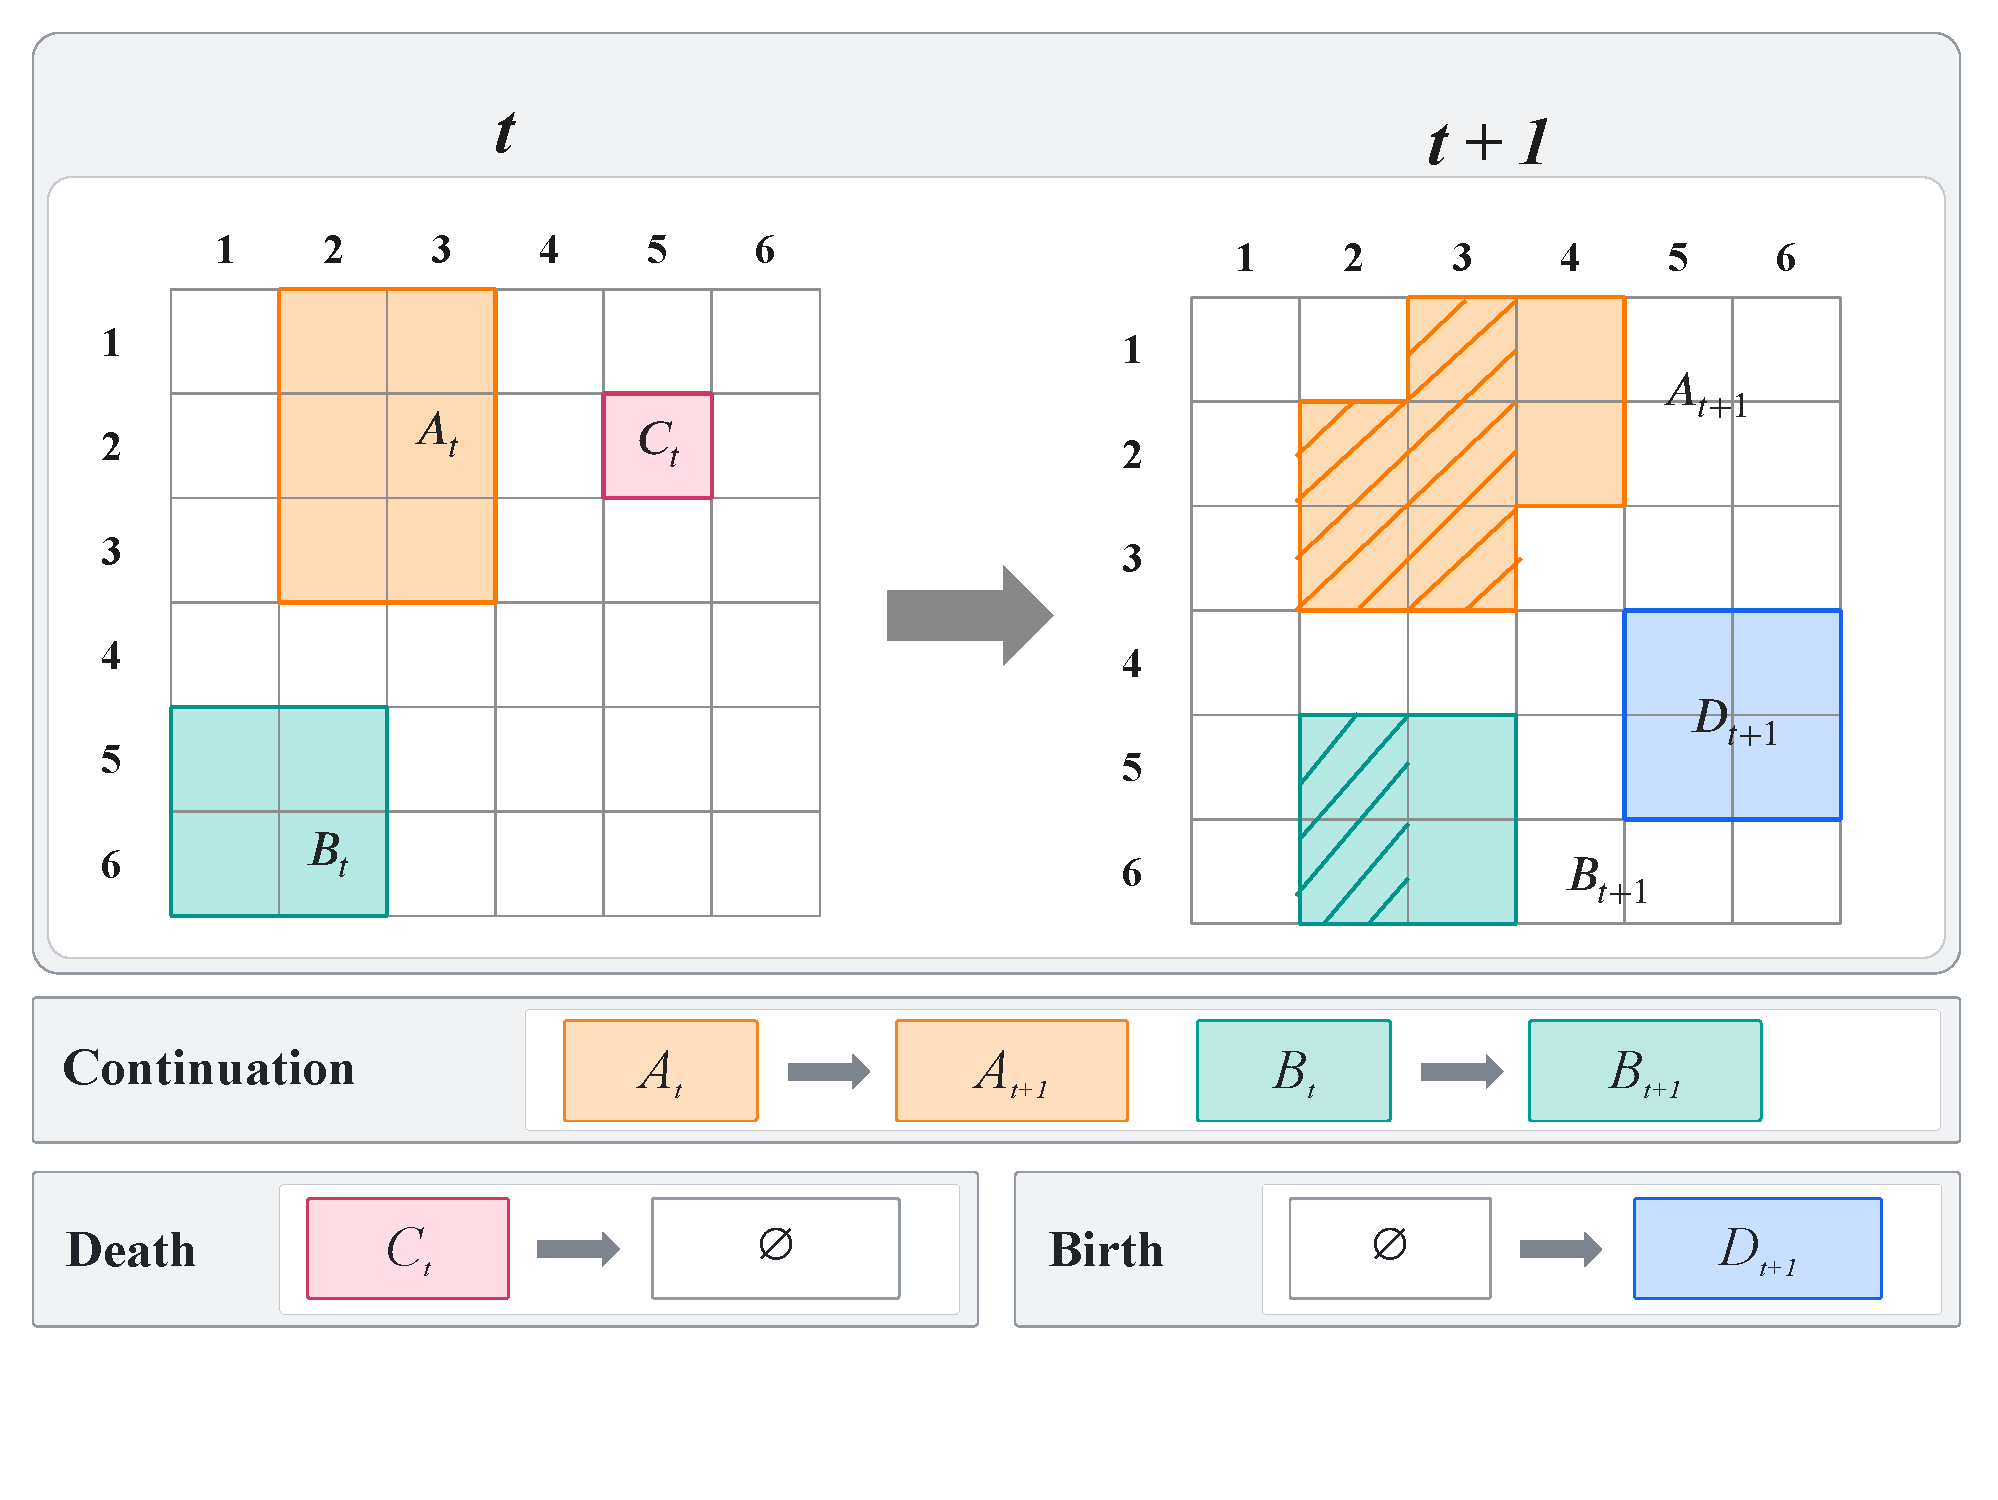
\includegraphics[width=0.7\linewidth]{figures/anchor_leaf_correspondence.pdf}
\caption{共享网格上基于重叠的叶对应。彩色区域表示叶弧支撑；阴影标出与前一帧共享的采样点。最大重叠的一对一分配使 $A$ 和 $B$ 延续，$C_t$ 未被匹配，并给 $D_{t+1}$ 分配一个新身份。出生和消亡表示匹配状态，而不是被识别出的物理事件。}
\label{fig:leaf_correspondence}
\end{figure}

这些对应关系在任何拓扑预算扫描之前计算，为空间锚定提供运动样本；空间锚定区分参考目标 $q_i^t$ 和显示锚点 $x_i^t$。
只有有效的相邻帧匹配才贡献位移；匹配失败或轨迹中断在该步不贡献样本。
默认情况下，用所有匹配的相邻帧极值位移，离线估计一个单位方向 $a^*\in\mathbb{R}^d$，$d\in\{2,3\}$：
\begin{equation}\label{eq:autodirection}
\begin{aligned}
 \Delta p_i^t&=p_i^t-p_{\mu_t(i)}^{t-1},\\
 S&=\sum_{t,i\;\mathrm{matched}}\Delta p_i^t(\Delta p_i^t)^\top,\\
 a^*&\in\arg\max_{\|a\|=1}a^\top Sa.
\end{aligned}
\end{equation}
主特征向量最大化投影运动的平方和，而不是特征数量或拓扑相容性。
同一计算适用于二维和三维；它对整个序列只做一次。
其符号使带符号的总投影运动非负；当带符号运动接近零时，令绝对值最大的分量为正。
当运动能量可以忽略时，使用区域的最长轴（相等时取第一个轴）。
主特征值重复时，最大化方向不唯一；报告的特征值间隙指示这种不确定性。
给定的物理方向可以替代 $a^*$，而不改变布局。
重叠匹配可能漏掉快速移动的特征，或支撑变化大、重叠弱的特征，从而影响位移样本，进而影响估计的方向。

对于选定的方向，投影后区域包围盒各角点的最小值和跨度定义了共同的原点 $o$ 和范围 $L>0$。
参考为
\begin{equation}\label{eq:reference}
 q_i^t=\langle a^*,p_i^t\rangle-o\in[0,L].
\end{equation}
对同一个准备好的序列，方向、原点和尺度在所有帧和所有预算下保持不变。
实现中的数组存储 $[o,o+L]$ 上的原始投影；把参考和布局坐标都平移 $-o$ 就得到论文中的约定。
原点只减一次，求解器不会再减。
不同的极值可以有相同的投影坐标，同时保留各自的身份。
锚定是最小化受约束的偏差，而不是要求 $x_i^t=q_i^t$。

相对几何使用叶支撑质心之间的距离 $d_{ij}^t$。
它们不同于极值参考，因为支撑变化时质心可能移动，而极值保持不动。
自动参考的适配器显式提供极值；底层求解器也接受预先计算的参考，否则默认使用质心投影。
宽度 $W_i^t=s\,m_i^t$ 以固定尺度 $s$ 把正的支撑测度转换为宽度，不做逐帧归一化。

在对应关系和参考固定之后，一帧由叶序、极值锚点和标量剖面组成：
\begin{equation}\label{eq:mapframe}
 M_t=(\pi_t,x_t,\psi_t),\qquad\psi_t:[0,L]\to\mathbb{R}.
\end{equation}
我们追求与参考对齐的位置和运动，同时近似相对几何并控制显示出的拓扑。
区间布局集合 $\mathcal{L}(\pi)$ 要求以 $z_i$ 为中心、宽度为 $W_i$ 的区间位于画布内，彼此不相交且间隙至少为 $g\ge0$，并包含满足 $|x_i-z_i|\le\rho W_i/2$（$0\le\rho\le1$）的锚点。
总宽度和间隙不可行时会被报告，而不是被重新缩放。

实际位移为 $|x_i-q_i|$，报告时除以 $L$ 归一化。
为了区分顺序冲突与有限宽度放置，定义
\begin{equation}\label{eq:nroe}
 \nroe(\pi)=\frac{1}{2L}\max_{j\le k}
                      [q_{\pi(j)}-q_{\pi(k)}]^+.
\end{equation}
这是非递减的点放置的最小最坏位移除以 $L$；它不考虑宽度。
对于有限区间，精确的固定叶序代价为
\begin{equation}\label{eq:tau}
 \tau(\pi)=\min_{(x,z)\in\mathcal{L}(\pi)}\|x-q\|_\infty.
\end{equation}
只要布局集合非空，最小值就能达到。
它由固定叶序的装箱约束精确计算，等价于一个极小极大线性规划。
对于不同的标签，令 $V_{ij}^{\psi}$ 为两锚点之间剖面的最大值，并令 $V_{ii}^{\psi}=\psi(x_i)$。
我们要求
\begin{equation}\label{eq:dtop}
\begin{aligned}
 \dtop(\psi_t,T_t)&=\max_{i,j}|V_{ij}^{\psi_t}-V_{ij}^t|\le\eta,\\
 \eta&=(\varepsilon_0+\varepsilon)\Delta_F.
\end{aligned}
\end{equation}
这里 $\Delta_F>0$ 是整个序列的标量值域，$\varepsilon_0$ 是固定的数值容差，$\varepsilon\ge0$ 是唯一的主要用户控制量。
实现默认 $\varepsilon_0=10^{-7}$。
没有 20\% 的上限：100\% 既不是数学上的上界，也不一定意味着拓扑完全不受限。
NMLE 报告实际达到的归一化误差 $\dtop/\Delta_F$。
精确拓扑意味着在给定的树上带标签误差为零。
非零的平局容差计入 $\eta$。

其余所有设置都属于一个固定配置 $\Theta_0$：位置余量 $\beta_0$、四个目标权重、宽度尺度、间隙、锚点余量和输出分辨率。
对一个准备好的序列，默认接口为 $M_t^\varepsilon=\operatorname{AnchorMTM}(T_t,q_t,W_t,V_t,\mu_t;\varepsilon,\Theta_0)$。
高级设置可以一次性给定，但在预算扫描中只改变 $\varepsilon$。
补充材料给出了固定的尺度规则和实现容差。

对于固定标签覆盖每一片叶子、且诱导矩阵包含对角线的标准同表型合并树表示，$\dtop$ 等于未归一化的带标签交错距离~\cite{Munch:2019:LINF,Gasparovic:2024:IID}。
在这些条件下，$d_B\le d_I\le\dtop$~\cite{Morozov:2013:IDMT}。
在把这一解释用于整个显示出的树之前，必须检查渲染引入的无标签极值。

\subsection{空间锚定布局的构造}\label{sec:construction}
在特征及其参考固定之后，构造按字典序目标选择叶序：
\begin{equation}\label{eq:orderobjective}
\begin{aligned}
 \pi_t^\varepsilon&\in\underset{\pi\in\mathcal{C}_t(\varepsilon)}{\arg\min}
                    \bigl(\tau_t(\pi),\nroe_t(\pi)\bigr),\\
 &\hspace{1em}\mathrm{s.t.}\quad\delta_t^*(\pi)\le\eta(\varepsilon).
\end{aligned}
\end{equation}
有限的候选池包含原始的严格拓扑叶序、中点初始化，以及在阈值展平和选择性展平的宽度感知细化过程中访问过的叶序。
每个候选都用同一个源合并矩阵评估。
选择时先最小化 $\tau$，再最小化 NROE；它不是在全部排列上的全局最优。
算法~\ref{alg:construction} 把这一离散选择与固定叶序下的放置分开。

\begin{algorithm}[htbp]
\caption{单一控制量的 AnchorMTM}\label{alg:construction}
\KwData{二维/三维场序列及网格；$\varepsilon\ge0$；固定配置 $\Theta_0$。}
\KwResult{时间地图 $I^\varepsilon$、误差记录或失败报告。}
提取增广树、叶支撑和极值；匹配支撑并分配轨迹 ID\;
估计一个方向和固定参考 $q_t$；在各预算间复用这一预处理\;
$\eta\leftarrow(\varepsilon_0+\varepsilon)\Delta_F$\;
\For{按时间顺序的每个时间步 $t$}{
 若宽度和间隙超出固定画布，则报告并停止\;
 $\mathcal{C}_t\leftarrow\operatorname{GenerateAndRefine}(T_t,q_t,W_t,V_t,\eta)$；保留严格拓扑候选\;
 对候选计算 $\tau(\pi)$、$\nroe(\pi)$ 和 $\delta^*(\pi)$\;
 $\mathcal{F}_t\leftarrow\{\pi\in\mathcal{C}_t:\delta^*(\pi)\le\eta\}$\;
 \lIf{$\mathcal{F}_t=\varnothing$}{报告无可行候选并停止}
 按 $(\tau,\nroe)$ 从 $\mathcal{F}_t$ 中选出 $\pi_t^\varepsilon$\;
 为 $\pi_t^\varepsilon$ 计算最优合并屏障\;
 只对 $\pi_t^\varepsilon$ 求解四项二次规划，上限为 $\tau(\pi_t^\varepsilon)+\beta_0$，并使用有效的匹配历史\;
 通过叶/最近公共祖先填充和屏障修正重建剖面\;
 记录候选数量、连续误差与渲染误差、运动和失败；把剖面加入 $I^\varepsilon$\;
}
\KwReturn{$I^\varepsilon$ 及诊断记录}\;
\end{algorithm}

\subsubsection{拓扑预算下的叶序选择}
\emph{精确模式}令 $\eta=0$，要求在给定的树上带标签合并误差为零。
\emph{预算模式}允许 $\eta>0$。
只把附加预算设为 $\varepsilon=0$ 而保留 $\varepsilon_0>0$，得到的是数值容差，而不是零带标签误差。
两种模式共享同一个区间模型和放置目标。

候选生成包括精确的树、阈值展平和一种由冲突驱动的选择性展平。
中点叶序初始化这些结构。
宽度感知的块插入细化最好的四个初始结构以及精确的树，同时保留点模型的预算叶序作为候选。
移动步骤改进由 $\tau$ 和装箱残差平方项构成的字典序得分，并且必须通过 $\delta^*(\pi)\le\eta$。
访问过的初始叶序和试探叶序都保留在去重后的候选池中，包括严格树初始化和保留的点候选。
最终的预算过滤和字典序选择使用精确的固定叶序代价；细化过程不保证在全部排列上的全局最优。

保护机制会报告容量失败、空的可行集合和求解器失败，而不会悄悄地重新缩放宽度、间隙或画布；细节见补充材料。

\subsubsection{最优合并屏障与拓扑可行性}
对于固定叶序，一对叶子显示出的合并值是它们之间最大的屏障。
对间隙 $k$，令 $C_k=\min_{i\le k<j}V_{\pi(i)\pi(j)}$，$F_k=\max(V_{\pi(k)\pi(k)},V_{\pi(k+1)\pi(k+1)})$。
\begin{proposition}[最优屏障]\label{prop:barriers}
在极值固定、连续、非严格的模型中，最小的带标签合并误差为
\begin{equation}\label{eq:delta}
\begin{split}
 \delta^*(\pi)=\max\bigg\{&0,\max_k(F_k-C_k),\\
 &\frac12\max_{i<j}\left(V_{\pi(i)\pi(j)}-
                         \max_{i\le k<j}C_k\right)\bigg\},
\end{split}
\end{equation}
并且屏障 $b_k=C_k+\delta^*(\pi)$ 能达到它。
\end{proposition}
误差 $\delta$ 要求 $F_k\le b_k\le C_k+\delta$。
当 $\delta\ge\delta^*$ 时，选择最大的允许屏障恰好满足每一对的合并下限要求。
因此，在这个连续模型中，叶序满足合并允许量当且仅当 $\delta^*(\pi)\le\eta$。
这一固定叶序检验支撑候选搜索，但并不使搜索全局最优。
严格极值的余量和栅格效应单独检查。

\subsubsection{空间锚定的时空放置}
叶序固定后，核心项是 $E_R$（与固定参考偏差的均方）和 $E_M$（匹配的投影运动的均方误差）。
辅助项 $E_G$ 通过有序锚点间距来近似支撑质心之间的距离；$E_C$ 约束锚点偏离区间中心的程度。
四项及其非负权重全部保留：
\begin{equation}\label{eq:qp}
\begin{aligned}
 \min_{x_t,z_t}\quad&\lambda_R E_R+\lambda_G E_G+\lambda_M E_M+\lambda_C E_C\\
 \mathrm{s.t.}\quad&(x_t,z_t)\in\mathcal{L}(\pi_t),\\
 &\|x_t-q_t\|_\infty\le\tau(\pi_t)+\beta_0.
\end{aligned}
\end{equation}
对每个有效匹配，令 $\Delta q_i^t=q_i^t-q_{\mu_t(i)}^{t-1}$，并以前一帧的显示锚点加上这一参考位移作为时间目标：
\begin{equation}\label{eq:temporal_target}
 \hat x_i^t=x_{\mu_t(i)}^{t-1}+(q_i^t-q_{\mu_t(i)}^{t-1}).
\end{equation}
因此 $E_M$ 追随投影运动，同时偏好 $x-q$ 的连续性。
第一帧、新出生的叶子以及其他未匹配的叶子没有前一帧运动惩罚。
每一项都在其特征、有序对或有效匹配上取平均；当前的自动参考适配器对有效匹配使用单位置信度。
补充材料区分了这一默认设置与旧的按置信度加权的路径。

只有 $\varepsilon$ 改变拓扑允许量 $\eta(\varepsilon)$。
固定余量 $\beta_0\ge0$ 限制排序之后额外的位置偏差。
由于 $\tau(\pi_t)$ 能够达到，这个上限是可行的；二次规划只接收所选叶序，不能把它换成二次目标更低的其他叶序。
它限制连续位移，而几何和时间目标在这个上限内选择一个折中。
固定叶序下的问题是凸的；逐帧顺序处理并不意味着整个序列的联合最优，也不意味着精确保持每一个投影运动。

\subsubsection{剖面重建与输出诊断}
重建沿用合并树图流程中的叶弧采样和最近公共祖先路径填充~\cite{Koepp:2023:TMTM,STMTM:2026}。
原始极值保留在其锚点上；正则采样点在区间和间隙中提供标量背景。
随后，最优屏障修正把每个锚点之间的内部截断到 $b_k$，必要时抬高已有的峰。
放松后的叶序需要这一单独的修正；仅靠继承的最近公共祖先填充无法保证极小极大屏障。

所有帧使用共同的方向、原点、范围和像素换算。
这些剖面构成最终的时间地图：
\begin{equation}\label{eq:map}
 I^\varepsilon(t,u)=\psi_t^\varepsilon(u),\qquad 0\le u\le L.
\end{equation}
不做逐帧的重新居中。
重采样不会保留每一个源采样点，严格极值的余量和栅格取整可能改变实际达到的误差；重建失败和完整树的标签覆盖按补充材料所述检查。
因此，一个记录下来的剖面并不能仅凭 $\delta^*\le\eta$ 就被无条件地证明。
记录区分所请求的预算、位置证书、实际达到的 $\tau$、连续的 $\delta^*$ 和实际渲染误差。

\subsection{可证明的位置–拓扑界}\label{sec:bounds}
即使经过优化，构造仍可能留下参考位移。
下面的界解释了拓扑和有限宽度使哪些位移不可避免：第一个回答与树相容的点叶序必须偏离多少，第二个加入区间装箱，第三个问在合并误差允许量下还剩哪些限制。
它们是分析性的基准，不是三个执行阶段，也不是搜索剪枝规则；构造使用精确的固定叶序代价 $\tau$ 和 $\delta^*$。
由此得到的证书与布局算法无关。
完整证明和计算定义见补充材料。
在一帧之内我们省略 $t$，记 $[v]^+=\max(v,0)$，并约定空集上的最大值为零。

\subsubsection{精确拓扑下的参考顺序界}
对于真祖先高度严格递增的约简树，精确拓扑使每棵子树连续。
令 $[m_X,M_X]$ 为子树 $X$ 中叶子的参考包络。
\begin{theorem}[精确拓扑位置界]\label{thm:order}
每一个零误差的剖面都满足 $\nroe(\pi)\ge\nu^*(T,q)$，其中
\begin{equation}\label{eq:nu}
 \nu^*(T,q)=\frac{1}{2L}\max_v\max_{\substack{X,Y\in\mathrm{ch}(v)\\X\ne Y}}
 [\min(M_X-m_Y,M_Y-m_X)]^+.
\end{equation}
按参考包络中点递归地对子结点排序，能在 $O(n\log n)$ 时间内达到这个点模型顺序界。
\end{theorem}
\begin{proof}[证明概要]
兄弟块必须选择一种朝向。
两种朝向可能的反序代价分别为 $[M_X-m_Y]^+/2$ 和 $[M_Y-m_X]^+/2$。
中点排序选择较小者；每一对反序的叶子都在其最近公共祖先处被兄弟块分开。
\end{proof}
这一结果孤立出树和参考所施加的排序限制。
中点排序达到点叶序的最优；有限区间引入额外的约束，接下来讨论。

\subsubsection{宽度感知的位置界}
有限宽度、最小间隙、锚点余量和画布容量在点叶序的阻碍之上增加了装箱代价。
对非空叶子集合 $S$，令 $H_i=\rho W_i/2$，$\ell_i=q_i-W_i/2-H_i$，$h_i=q_i+W_i/2+H_i$，$s_i=W_i+g$。
定义两个装箱量：
\begin{equation}\label{eq:packing}
\begin{aligned}
 A(S)&=\max_{a\in S}\left(\ell_a+\sum_{\substack{i\in S\\\ell_i\ge\ell_a}}s_i\right),\\
 B(S)&=\max_{b\in S}\left(\sum_{\substack{i\in S\\h_i\le h_b}}s_i-h_b\right).
\end{aligned}
\end{equation}
前者使用上参考端点集合，后者使用下集合；排序和累加和即可计算。
对不相交的叶子集合 $X,Y$ 和全体叶子集合 $\mathcal{F}$，记
\begin{equation}\label{eq:packingcost}
\begin{aligned}
 \omega(X,Y)&=\tfrac12\min\{A(X)+B(Y),A(Y)+B(X)\}-\tfrac g2,\\
 E_\partial&=\max\{0,B(\mathcal{F})-g,A(\mathcal{F})-g-L\}.
\end{aligned}
\end{equation}
其中 $\omega$ 取代价较低的块朝向，$E_\partial$ 考虑画布的两端。
令 $\mathcal{P}_0$ 包含所有不同兄弟后代叶集合的配对。
证书为
\begin{equation}\label{eq:bwdef}
 \mathcal{B}_w(T,q,W)=\max\{E_\partial,\max_{(X,Y)\in\mathcal{P}_0}\omega(X,Y)\}.
\end{equation}
对 $g$、$\rho$ 和 $L$ 的依赖通过式~\ref{eq:packing}–\ref{eq:packingcost} 体现，在证书的自变量中省略。
\begin{theorem}[宽度感知位置界]\label{thm:width}
对任意可行的精确拓扑区间布局，
\begin{equation}\label{eq:widthbound}
 \|x-q\|_\infty\ge\tau(\pi)\ge\mathcal{B}_w(T,q,W).
\end{equation}
当宽度和间隙为零时，$\mathcal{B}_w=L\nu^*(T,q)$。
\end{theorem}
\begin{proof}[证明概要]
所选叶子的第一个和最后一个锚点必须包住它们的区间和其间的间隙（在允许的锚点余量之内）。
式~\ref{eq:packing} 中的上、下集合使由此产生的相对于参考间隔的不足量最大。
精确拓扑要求每一对兄弟只能有一种朝向；画布两端给出两个单侧代价。
\end{proof}
因此 $\mathcal{B}_w$ 是所有精确拓扑合法区间叶序的下界，且不一定能达到；$\tau(\pi)$ 是给定叶序下实际达到的最小值。
这些量以坐标为单位，而 NROE 和 $\nu^*$ 用 $L$ 归一化。

\subsubsection{有限拓扑误差下的位置界}
合并值允许量可以解除一部分连续块，但仍然限制交错。
如果叶 $k$ 位于结点 $u$ 的两个后代 $i,j$ 之间，区间包含关系给出 $V_{ik}^{\psi}\le V_{ij}^{\psi}$，从而 $V_{ik}\le h(u)+2\eta$。
定义 $A_\eta(u)$ 为满足 $h(A_\eta(u))-h(u)\le2\eta$ 的最高祖先（包括 $u$ 自身）。
这里使用标量单位下累计的祖先高度差，作用在约简后的等高树上，并使用式~\ref{eq:dtop} 的固定标签。

令 $\mathcal{P}_\eta$ 由两类叶集合配对组成：对每个内部结点 $u$ 和叶 $k\notin\mathcal{D}(A_\eta(u))$ 的 $(\mathcal{D}(u),\{k\})$；以及满足下式的内部结点 $u,w$ 的 $(\mathcal{D}(u),\mathcal{D}(w))$：
\begin{equation}\label{eq:separatedpairs}
\begin{aligned}
 \mathcal{D}(w)\cap\mathcal{D}(A_\eta(u))&=\varnothing,\\
 \mathcal{D}(u)\cap\mathcal{D}(A_\eta(w))&=\varnothing.
\end{aligned}
\end{equation}
对任意非空叶集合 $X$，使用其参考包络 $[m_X,M_X]$，并定义 $\kappa(X,Y)=[\min(M_X-m_Y,M_Y-m_X)]^+/(2L)$。
两个证书为
\begin{equation}\label{eq:chaindef}
\begin{aligned}
 C_\eta(T,q)&=\max_{(X,Y)\in\mathcal{P}_\eta}\kappa(X,Y),\\
 C_{w,\eta}(T,q,W)&=\max\{E_\partial,\max_{(X,Y)\in\mathcal{P}_\eta}\omega(X,Y)\}.
\end{aligned}
\end{equation}
\begin{theorem}[有限拓扑误差位置界]\label{thm:chain}
在 $\dtop\le\eta$ 的剖面中，$\mathcal{D}(A_\eta(u))$ 之外的叶子不能位于 $u$ 的两片叶子之间。
$\mathcal{P}_\eta$ 中的每一对都整体处于一种块朝向或另一种。
因此
\begin{equation}\label{eq:chainbounds}
 \nroe(\pi)\ge C_\eta(T,q),\qquad
 \tau(\pi)\ge C_{w,\eta}(T,q,W),
\end{equation}
其中第二个不等式适用于区间模型。
\end{theorem}
分离原理排除了每一对符合条件的配对之间的交错；两种可能的朝向分别给出 $\kappa$ 和 $\omega$。
因此 $C_\eta$ 是归一化参考顺序误差的下界，而 $C_{w,\eta}$ 以坐标为单位包含了有限宽度和边界代价。
累计的祖先间隙使这些证书至少与“展平所有不超过 $2\eta$ 的父间隙”所得的证书一样强。

允许量针对的是显示出的层次；源场和特征身份保持不变。
更大的可行集合不一定改进每一个特征或每一个启发式结果。
这些界作为不可避免误差的基准来报告；排序和连续意义下的接受使用第~\ref{sec:construction} 节中精确的固定叶序评估。
连续可行性不能保证完整渲染出的栅格。

\subsection{已有合并树图是同一公式的特例}\label{sec:special}
上述构造是一个更一般公式的一个实例。
我们考虑的每一种合并树图，都在每帧选择叶序、区间布局和剖面，求解
\begin{equation}\label{eq:general}
\begin{aligned}
 \min_{\{M_t\}}\quad&\textstyle\sum_t\lambda_O E_O+\lambda_G E_G+\lambda_M E_M+\lambda_R E_R+\lambda_C E_C+\lambda_W E_W\\
 \mathrm{s.t.}\quad&\pi_t\in\Pi_\eta(T_t),\quad (x_t,z_t)\in\mathcal{L}(\pi_t),\quad \|x_t-q_t\|_\infty\le B_t,
\end{aligned}
\end{equation}
其中 $\Pi_\eta(T_t)$ 包含最优屏障满足允许量（即 $\delta_t^*(\pi)\le\eta$）的叶序，$E_O$ 是 TMTM 的子树重叠项，$E_W$ 是 ST-MTM 的宽度偏差项，$E_G,E_M,E_R,E_C$ 是式~\ref{eq:qp} 中的各项。
允许量 $\eta$、位置上限 $B_t$、选择 $\pi_t$ 的规则和目标权重共同决定一张图（表~\ref{tab:instances}）。
TMTM 和 ST-MTM 是精确拓扑的特例，没有位置上限，也没有参考项；投影是允许量无限的特例，其叶序就是参考顺序；AnchorMTM 固定了参考项和上限，并把允许量作为唯一的控制量。

\begin{table}[tbp]
\caption{作为式~\ref{eq:general} 特例的合并树图。}\label{tab:instances}
\centering\small
\begin{tabular}{lllll}\toprule
图 & 允许量 $\eta$ & 上限 $B_t$ & 排序规则 & 目标\\\midrule
TMTM~\cite{Koepp:2023:TMTM} & $0$ & $\infty$ & 贪心子树翻转 & $E_O$\\
ST-MTM~\cite{STMTM:2026} & $0$ & $\infty$ & 空间邻近 & $E_G+\lambda_M E_M$；$E_W$\\
投影 & $\infty$ & $\tau_t+\beta_0$ & 按 $q$ 排序 & 式~\ref{eq:qp}\\
AnchorMTM & $(\varepsilon_0+\varepsilon)\Delta_F$ & $\tau_t+\beta_0$ & 算法~\ref{alg:construction} & 式~\ref{eq:qp}\\\bottomrule
\end{tabular}
\end{table}

第~\ref{sec:bounds} 节的界只依赖于式~\ref{eq:general} 的约束，而不依赖于目标函数或求解器，因此能衡量所有满足其假设的特例。
定理~\ref{thm:order} 对每一张精确拓扑的图都成立，无论其宽度规则或求解器如何，因此也适用于 TMTM 和 ST-MTM。
定理~\ref{thm:width} 适用于区间模型 $\mathcal{L}$ 中的精确拓扑图，ST-MTM 和 AnchorMTM 都属于这一模型；定理~\ref{thm:chain} 适用于每一张合并误差不超过 $\eta$ 的图。
因此，对任何精确拓扑的图，高于 $\nu^*$ 的顺序误差都是由其排序规则造成的，而不是由数据造成的；第~\ref{sec:experiments} 节对此进行测量。

\section{实验}\label{sec:experiments}
实验检验框架的三个主张：锚定消除了精确地图中可以避免的顺序误差（第~\ref{sec:anchoring} 节），界识别出剩下的部分（第~\ref{sec:bounds-eval} 节），$\varepsilon$ 在其允许量内描出位置–拓扑权衡（第~\ref{sec:tradeoff} 节）；第~\ref{sec:cases} 节和第~\ref{sec:ablation} 节给出案例研究、排序及其代价。

\subsection{实验设置}\label{sec:setup}
\paragraph{数据。}
基准包括七个序列共 917 帧（表~\ref{tab:data}）：平面区域上的再分析气压、卫星辐射、火灾排放和空气质量数据，两个三维流动模拟，以及 TMTM 的合成序列 Ring~\cite{Hersbach:2020:ERA5,Franke:2021:1DP,NOAA:OLR,Dong:2026:PM25,Koepp:2023:TMTM,Popinet:2004:Tangaroa,Camarri:2005:Cylinder,Weinkauf:SquareCylinder}。
所有图共享处理后的场、增广合并树、叶支撑、跨帧对应和参考坐标。
参考按式~\ref{eq:reference} 构造：在 Tangaroa 上，方向是估计的运动方向（式~\ref{eq:autodirection}）；在 Storms 和 Cylinder 上，我们给定具有物理意义的东西向轴和顺流轴。
另有两个序列只用于展示，不进入任何基准汇总：图~\ref{fig:storms_overview} 中 744 帧的逐小时 Storms 场，以及一个 90 帧的三维 Vortex 序列。

\begin{table}[tbp]
\caption{基准序列。叶子：每帧保留的极值数。}\label{tab:data}
\centering\small
\begin{tabular}{llrrl}\toprule
序列 & 标量场 & 帧数 & 叶子 & 树\\\midrule
Storms & ERA5 平均海平面气压，二维 & 118 & 1--8 & 并树\\
Wildfires & $\log(1+\mathrm{FRP})$，二维 & 30 & 6--11 & 分裂树\\
OLR & 射出长波辐射，二维 & 60 & 2--8 & 并树\\
PM$_{2.5}$ & PM$_{2.5}$ 浓度，二维 & 366 & 1--7 & 分裂树\\
Ring & 合成环形强度，二维 & 40 & 1--7 & 分裂树\\
Tangaroa & 速度大小，三维 & 201 & 18--93 & 并树\\
Cylinder & Q 判据，三维 & 102 & 4--75 & 分裂树\\\bottomrule
\end{tabular}
\end{table}

\paragraph{特例。}
我们评估表~\ref{tab:instances} 中的四个特例。
AnchorMTM 以默认配置 $\Theta_0$ 运行精确模式（$\varepsilon=0$，数值平局容差 $\varepsilon_0=10^{-7}$）和预算模式（除另行说明外 $\varepsilon=10\%$）。
TMTM 和 ST-MTM 用其原生输出评估；ST-MTM 没有公开代码，我们使用按其发表描述实现的版本。
给定原生叶序时，我们对式~\ref{eq:general} 的实现复现了这两种方法：TMTM 的线性化在全部 3127 个弧区间和锚点上与官方实现一致，ST-MTM 的锚点满足其二次规划的最优性条件（相对 KKT 残差低于 $10^{-6}$）。
即使对它们自己的目标，两种排序规则也都是启发式的：ST-MTM 的叶序在 10 帧上没有达到穷举最优，TMTM 的贪心选择比逐步最优高出最多 85.5\%。

\paragraph{指标。}
位置用 NROE（式~\ref{eq:nroe}）衡量，它只按顺序比较原生尺度不同的图；对区间模型中的图，还用 $|x_i-q_i|/L$ 在全部特征–帧上的汇总平均 $E_{\mathrm{pool}}$ 和最坏值 $E_\infty$ 衡量。
拓扑用 NMLE 衡量，即渲染后的 $\dtop/\Delta_F$（式~\ref{eq:dtop}）。
运动误差（ME）是明确的靠近或远离事件（即两个匹配极值在两步内二维或三维距离的变化）中，被地图显示成相反方向或完全没有显示的比例。
为了体现 ST-MTM 的目标，我们还按其协议报告锚点距离相对于支撑质心距离的尺度归一化应力（SNS）和可信度（TW，$k=1$）~\cite{STMTM:2026}；用保存的原生锚点重新计算，与存储的基线数值的相对误差在 $10^{-5}$ 以内，并一致到小数点后第三位。

\subsection{空间锚定消除可以避免的顺序误差}\label{sec:anchoring}
\begin{figure}[tbp]
\centering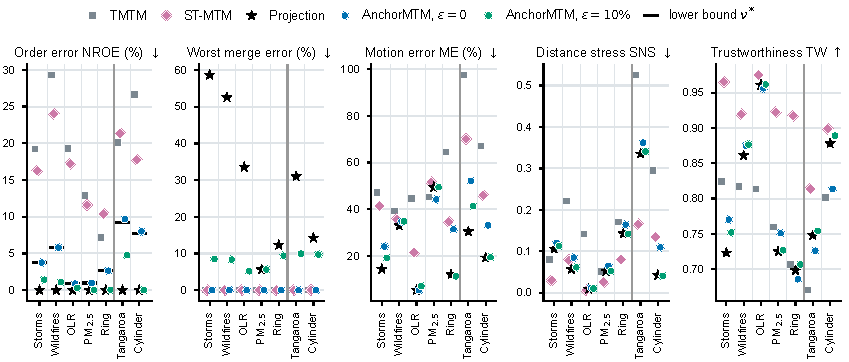
\includegraphics[width=\linewidth]{figures/fig_compare.pdf}
\caption{式~\ref{eq:general} 的各特例在七个序列上的表现（灰线左侧为平面，右侧为三维）。顺序误差 NROE 及定理~\ref{thm:order} 的精确拓扑下界 $\nu^*$（黑色短线）、渲染后的最坏合并误差、运动误差，以及距离指标 SNS 和 TW。精确拓扑的特例（TMTM、ST-MTM、$\varepsilon=0$ 的 AnchorMTM）合并误差为零；投影的顺序误差为零，但合并误差最高达 59\%。全部数值见补充材料。}\label{fig:compare}
\end{figure}

\emph{已有合并树图的大部分顺序误差是可以避免的，精确模式在不放弃合并树的前提下消除了它。}
由于 TMTM 和 ST-MTM 是精确拓扑的特例，定理~\ref{thm:order} 把它们的顺序误差分成层次强制的部分 $\nu^*$ 和由其排序规则选择造成的超出部分（图~\ref{fig:compare}）。
在七个序列上，超出部分占 TMTM 顺序误差的 54–95\%，占 ST-MTM 的 57–95\%；例如在 Storms 上，TMTM 的 19.2\% 中有 3.8\% 是层次强制的，而 ST-MTM 的 16.3\% 中有 12.5\% 不是。
精确模式在每个平面序列上都与 $\nu^*$ 相差不到 0.03 个百分点，且合并误差为零。
在 Tangaroa 上，宽度感知搜索接受略高的 NROE（9.67\% 对 9.24\%），以降低实际的最坏位移（第~\ref{sec:ablation} 节）。

\emph{锚定后的轴承载了运动。}
沿参考方向运动的特征现在在地图上也会移动，所以精确模式在全部七个序列上的运动误差都低于 TMTM 和 ST-MTM，例如 OLR 上 5.4\% 对 21.4\%，Tangaroa 上 52.2\% 对 70.0\%。
完全遵循参考顺序的投影在多数序列上运动误差更低，但这是以破坏树为代价的：它改变合并值最多达标量值域的 58.66\%（Storms）、52.58\%（Wildfires）、33.56\%（OLR）和 31.02\%（Tangaroa），在 Tangaroa 上没有任何一帧保持其树。
预算模式在其允许量内缩小了一部分这一差距（第~\ref{sec:tradeoff} 节）；没有任何渲染出的 AnchorMTM 地图超出其声明的允许量（数值容差内）。

\emph{获得空间轴的代价被明确报告，而不是被隐藏。}
锚定到一个方向，是用二维距离保持换取沿该方向的位置。
以成对距离为目标的 ST-MTM，在全部七个序列上 TW 最好，在五个序列上 SNS 最好。
当宽度起主导作用时，这种权衡可能反过来：在 Cylinder 上，预算模式的 SNS 为 0.041，而 ST-MTM 为 0.135。
在补充材料的地图中，精确模式把 OLR 的低辐射盆地放在参考附近，使地图可以和一张保留盆地嵌套关系的时间–经度图相比。

\subsection{可证明的界识别出剩下的位移}\label{sec:bounds-eval}
\begin{figure}[tbp]
\centering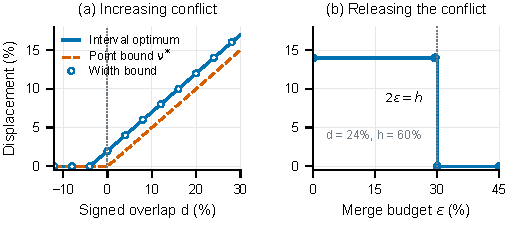
\includegraphics[width=0.6\linewidth]{figures/fig_controlled_conflict.pdf}
\caption{受控的四叶树。(a) 兄弟包络的重叠增大会迫使位移；圆圈标出定理~\ref{thm:width} 的宽度下界，穷举得到的区间最优恰好达到它。(b) 在重叠 $d=24\%$ 时，14\% 的区间位移只有在合并预算达到父间隙 $h=60\%$ 的一半时才消失，与定理~\ref{thm:chain} 的预测一致。百分比均相对于单位画布或单位标量值域。}\label{fig:controlled}
\end{figure}

\begin{figure}[tbp]
\centering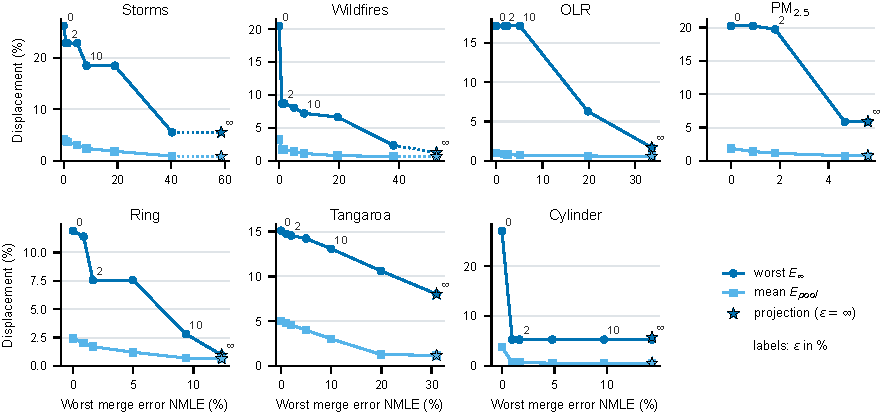
\includegraphics[width=\linewidth]{figures/fig_frontier.pdf}
\caption{由单一控制量 $\varepsilon$ 描出的位置–拓扑权衡。每个点是在预算 $\varepsilon$（标签，单位为百分比）下全部帧的一张图，按其渲染后的最坏合并误差和最坏位移（深色）、平均位移（浅色）摆放。星号：投影（$\varepsilon=\infty$）。}\label{fig:frontier}
\end{figure}

\emph{每个界孤立出一种位移来源。}
为了区分来源，我们固定两对兄弟 $X=\{A,B\}$ 和 $Y=\{C,D\}$：它们在 $0.4$ 处合并，根在 $1$，叶值为 $0$，单位画布上的参考为 $(0.2,0.5,0.5-d,0.8-d)$，带符号重叠 $d$ 从 $-0.12$ 变到 $0.30$。
在 43 个重叠值和四种宽度下，我们把这些界与全部 24 个叶序比较，每个叶序都用独立的极小极大线性规划放置。
仅拓扑一项就恰好强制 $\nu^*=\max(0,d)/2$。
在宽度 $W=0.06$、间隙 $0.01$、$\rho=0.5$ 时，宽度下界、我们的搜索和穷举最优三者重合于 $\tau=\max(0,(d+0.04)/2)$（图~\ref{fig:controlled}a）：在 $d=0.24$ 时分别为 12\% 和 14\%。
合并允许量恰好在定理~\ref{thm:chain} 允许交错的地方消除冲突，即在所测试的全部四个父间隙下都在 $2\varepsilon=h$ 处（图~\ref{fig:controlled}b）。
这些是受控实例，不是对一般紧度的断言。

\emph{在真实的树上，这些界仍然有信息量。}
宽度下界在多数平面帧上、以及 Tangaroa 和 Cylinder 的最坏帧上都能达到，但并非处处达到：在 Wildfires 的 $\varepsilon>0$ 情形和 OLR 在 $\varepsilon=10\%$ 时的一帧上，仍留有最坏帧的差距。
累计祖先间隙使有限误差下的界在大树上仍然有用：在 Tangaroa、$\varepsilon=5\%$ 时，把所有低于 $2\eta$ 的间隙展平只能证明平均 0.38\%，而带宽度的定理~\ref{thm:chain} 证明了 7.40\%，实际达到 8.10\%。
在 $\varepsilon=0$ 时也剩下相近大小的差距，这说明松的是界，而不是搜索。
因此，这些证书逐帧告诉分析者：一张图的位移中，有多少是模型中任何布局都无法避免的。

\begin{figure}[tbp]
\centering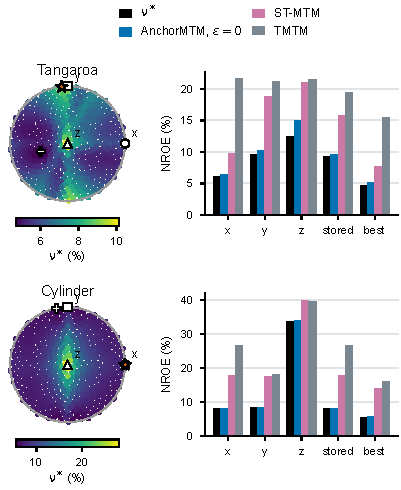
\includegraphics[width=0.55\linewidth]{figures/fig_direction_col.pdf}
\caption{在三维中选择参考。圆盘：半球上 400 个采样方向的平均顺序下界 $\nu^*$（等面积投影；圆心 $=z$ 轴，边缘 $=xy$ 平面）；标记依次为坐标轴、所存储的方向（星号；Tangaroa 上是估计的运动方向，Cylinder 上是顺流轴）和下界最小的方向（叉号）。柱状图：关键方向上的 $\nu^*$，以及精确模式、ST-MTM 和 TMTM 的平均顺序误差（原生朝向取对它们有利的一种）。}\label{fig:direction}
\end{figure}

\emph{由于这些界不需要先算出布局，它们可以在画图之前帮助选择参考。}
在三维中，投影丢掉两个坐标，所以不可避免的顺序误差取决于方向。
我们在两个三维序列上对 400 个采样方向计算了 $\nu^*$，参考按式~\ref{eq:reference} 构造（图~\ref{fig:direction}）。
在这些样本上，其平均值在 Tangaroa 上从 4.70\% 到 10.14\%，在 Cylinder 上从 5.26\% 到 28.15\%。
在 Tangaroa 上，估计的运动方向属于冲突最大的一类：400 个采样方向中只有 3 个下界更高，而改用 $x$ 轴可以把 $\nu^*$ 从 9.24\% 降到 6.09\%。
在 Cylinder 上，顺流轴位于中位数附近（7.72\%）。
在每个关键方向上，精确模式与下界相差不到 0.6 个百分点（唯一例外是 Tangaroa 的 $z$ 轴，相差 2.6 个百分点，那里宽度起主导作用），而 TMTM 和 ST-MTM 都远高于下界。

\subsection{一个控制量描出位置–拓扑权衡}\label{sec:tradeoff}


\emph{一个控制量覆盖从精确拓扑到参考顺序的整个权衡，而曲线在哪里转折取决于冲突的来源。}
图~\ref{fig:frontier} 描出每个序列从精确模式到投影的曲线；每个点都遵守其允许量。
冲突来自装箱时，小预算就够了：在 Cylinder 上，$\varepsilon=1\%$ 把最坏位移从 27.00\% 降到 5.27\%，低于投影的 5.73\%，因为按参考排序时没有考虑宽度；在 Wildfires 上，1\% 把 $E_\infty$ 从 20.48\% 降到 8.71\%；在 PM$_{2.5}$ 上，5\% 就已经达到投影的结果。
冲突来自强鞍点时，位置的代价很高：在 Storms 上，直到 $\varepsilon=20\%$，最坏位移都高于 18\%；在 OLR 上，有一帧直到 10\% 都保持 $E_\infty=17.14\%$。
预算只花在需要的地方：在 Storms、10\% 时，平均合并误差为 0.90\%，而最坏的一帧用了 8.51\%。

\emph{汇总上的改进并不等于逐点改进。}
在一个四叶对照中，在 $\varepsilon=30\%$ 时枚举全部 24 个叶序，最优最坏位移从 22\% 降到 1\%，但其中一个特征的误差从 0.087\% 升到 1\%。
在 Vortex 诊断序列上，把 $\varepsilon$ 从 20\% 提高到 30\%，汇总误差降了一半多（8.79\% 到 4.27\%），但 12,446 个特征–帧观测中有 30.91\% 变差，其中 24.72\% 变差至少 0.5 个百分点的 $L$。
记录下来的锚点和参考使这些局部变化可以在接受预算之前被检查。

\subsection{案例研究}\label{sec:cases}
\emph{Storms：一张读起来像地理的精确地图。}
在 118 帧的 Storms 基准上，极小值是穿过北大西洋的低压系统，参考是东西向轴。
以“每步最坏位移在各步上的平均值”衡量，在同一布局模型内，TMTM 和 ST-MTM 的目标把特征放在离参考 37.3\% 和 50.7\% 画布宽度的地方，精确模式为 5.1\%（中位数 0.8\%，少数几步峰值为 26.2\%）。
10\% 的预算把平均值降到 2.7\%；这份预算花在 118 步中的 31 步上，最多 8.51\%，平均 0.90\%，合并值变化超过标量值域 0.1\% 的 89 个屏障在地图上做了标记（见补充材料）。
图~\ref{fig:storms_overview} 以 $\varepsilon=5\%$ 和一个固定的投影方向，把这一构造应用到 1999 年 12 月的 744 个逐小时场上。
其快照跟踪一个匹配的极小值，即 12 月 16 日到 19 日斯堪的纳维亚上空的一个强风暴，它的显示位置在框出的时间窗内形成一条连续的轨迹；这条轨迹是叶特征之间的计算对应，本身并不能证明风暴在物理上的生成或消亡。



\emph{跨领域：平面和三维场用同一个构造。}
补充材料在三个平面序列和两个三维序列上，对每个数据集跟踪一个特征，跨越 18–41 个时间步，覆盖从 0 到 30\% 的六档预算，每一行保持同一个特征和参考。
对照参考轨迹阅读这些行，可以逐个特征看到更大的预算改变了什么，这是图~\ref{fig:frontier} 的汇总曲线无法显示的。

\subsection{排序与代价}\label{sec:ablation}
\paragraph{宽度感知排序。}
当特征很大时，对点最优的叶序不一定对区间最优。
在 Tangaroa 上，只按 NROE 排序（即点模型的预算叶序），在 $\varepsilon=0$ 时最坏位移为 20.69\%。
像算法~\ref{alg:construction} 那样按精确的区间代价 $\tau$ 对候选排序，把它降到 $\varepsilon=0$ 时的 15.10\% 和 $\varepsilon=2\%$ 时的 14.55\%，后者的最坏帧恰好达到下界；代价是平均时间跳动从 2.73\% 变为 2.82\%。
在 Cylinder 上，$\varepsilon\ge2\%$ 时，$E_\infty$ 从点模型叶序的 5.73\% 降到 5.27\%，同样达到下界。

\paragraph{搜索覆盖与运行时间。}
在全部 637 个叶子数不超过 8 的帧上，在 0 到 100\% 的九档预算下，有限搜索选出的叶序都等于穷举最优。
这些界的计算代价为 $O(n\log n)$ 到 $O(n^2\log n)$，$\delta^*$ 对每个叶序为 $O(n^3)$。
在一台 Apple M2 Pro 上（单个 Python 进程；NumPy 2.0、SciPy 1.13），全部界的计算在每个平面帧（1–11 片叶子）上最多 0.6\,ms，在每个三维帧（最多 93 片叶子）上最多 5.5\,ms；排序最多分别为 3.7\,ms 和 103\,ms；带上限的二次规划（SciPy SLSQP）分别为 2.3–9.0\,ms 和 0.25–0.50\,s。
全部 917 帧在 $\varepsilon=0$ 时用时 94\,s，有预算时最多 137\,s。

\section{讨论与局限}\label{sec:discussion}
\paragraph{合并树图的统一公式。}
把合并树图写成式~\ref{eq:general} 的特例，把已有方法隐含做出的三个决定分开了：显示轴表示什么（参考及其上限）、拓扑可以改变多少（允许量）、要保留哪些次要几何（目标）。
它也给每一张精确地图提供了一把共同的尺子：由于中点排序能达到 $\nu^*$，高于它的部分都是在设计上可以避免的；而宽度界和有限拓扑界不一定能达到，超出部分是从上方对“更好的布局能消除多少”的估计。

\paragraph{预算改变了什么。}
预算从不删除特征、不改变极值的值，也不移动数据。
在连续模型中，它改变合并值最多 $\eta=(\varepsilon_0+\varepsilon)\Delta_F$，我们测量的每张渲染地图都保持在这个允许量之内。
在标签覆盖全部叶子的地方（我们在 Ring 和 OLR 的 200 个渲染列上验证过），显示的树及其持续图与源数据之间的交错距离和瓶颈距离，都不超过测得的合并误差。
持续性简化则删除低于 $2\varepsilon$ 的特征~\cite{Edelsbrunner:2002:TPS,Tierny:2012:GTS}。
子树被拆开的地方，它的色带不再连续，“一条色带就是一个连通分量”的读法在局部失效，所以要标记这些屏障。

\paragraph{使用 AnchorMTM。}
结果提示了一个简单的流程。
第一，用 $\nu^*$（每帧几毫秒）比较候选参考，在估计的运动方向和具有物理意义的方向之间作选择。
第二，从精确模式开始：它在平面数据上的位置误差接近可证明的下界，合并树是精确的。
第三，扫描 $\varepsilon$，选择权衡曲线开始下降处的最小预算，并在接受之前检查被标记的屏障和逐特征残差。

\paragraph{局限。}
一个方向无法编码其余坐标：投影相同的特征会争夺同一个位置，而估计的方向追随主导运动，不一定是冲突最少的方向。
这个方向是离线地用全部匹配估计的；在线使用需要给定方向，或用更早一段时间拟合的方向。
构造继承了对应关系的质量：漏匹配或错误匹配会改变估计的方向和运动项。
叶序搜索是有限的启发式方法：在叶子数不超过 8 的所有帧上都与穷举一致；在更大的树上，它的超出部分只能由它与下界之间的差距来限制。
连续可行性不能保证渲染出的栅格：重采样、严格极值的余量和像素取整都可能改变实际的合并误差，因此我们把渲染误差与 $\delta^*$ 分开报告。
所有结果都使用默认配置 $\Theta_0$，我们没有研究它的敏感性。
位置是相对于 AnchorMTM 所追求的参考来测量的，因此我们也报告了原生输出的无尺度顺序误差和 ST-MTM 的距离指标；在这些指标上，ST-MTM 的 TW 仍然更好，SNS 在多数序列上更好。
最后，运动误差是假设特征身份已知的几何代理指标；分析者能否把位置和嵌套一起读出、披露标记能否防止误读~\cite{Kamakshidasan:2021:MM,McNutt:2020:SVM}，都需要用户研究来回答。

\section{结论}
AnchorMTM 赋予时间合并树图空间含义。
一个参考（由特征运动估计，或由分析者给定）把显示轴变成空间坐标；一个控制量决定为追随它可以改变多少拓扑；三个可证明的界说明精确拓扑、有限宽度和有限拓扑误差分别使多少位移不可避免。
由于已有合并树图是同一公式的特例，这些界也能衡量它们：在七个平面和三维序列上，它们的顺序误差有 54–95\% 是可以避免的，而精确模式在平面数据上几乎消除了全部这部分，且不改变合并树。
在数据允许的地方，预算能进一步改善位置，同时合并误差保持在声明的允许量之内，其改动也在图上标出。
下一步是面向大树的可扩展叶序搜索、超越单一方向的参考，以及一项关于同时判读位置和合并值的用户研究。

\bibliographystyle{abbrv-doi-narrow}
\bibliography{refs}
\end{document}
